

\section {Motivation}
\label{sec:motivation}

To date, two types of T2K oscillation analyses exist \cite{OurRun123DisappAnalysis3Flavour, NueRun123Analysis}:
\begin{itemize}
\item
  $\nu_{e}$-appearance analyses,
  in which $\sin^{2}2\theta_{13}$ and $\delta_{CP}$ are determined simultaneously using the SuperK single e-like ring event sample.
  In these analyses, the values of $|\Delta m_{32}^{2}|$ and $\sin^{2}2\theta_{23}$ are fixed
  and a neutrino mass hierarchy is assumed. To find the best-fit point and confidence interval for $\sin^{2}2\theta_{13}$, this type 
  of analysis typically fixes $\delta_{CP}$ to 0.0. The confidence region in the ($\sin^{2}2\theta_{13}$, $\delta_{CP}$) space is 
  usually calculated using a raster scan.
\item
  $\nu_{\mu}$-disappearance analyses, 
  in which $|\Delta m_{32}^{2}|$ and $\sin^{2}2\theta_{23}$ are determined simultaneously using the SuperK single $\mu$-like ring event sample.
  In these analyses, the values of $\sin^{2}2\theta_{13}$ and $\delta_{CP}$ are fixed
  and a neutrino mass hierarchy is assumed.
\end{itemize}

\noindent
However the oscillation parameters that are fixed have a non-negligible effect on P($\nu_{\mu}$$\rightarrow$$\nu_{\mu}$) and P($\nu_{\mu}$$\rightarrow$$\nu_{e}$), 
and this is shown in Fig.\ \ref{fig:oscprob}. 
The fixed oscillation parameters can also have a significant impact on the confidence regions, 
as demonstrated in Fig.\ \ref{fig:effectpriornuecontours} for the 
stand-alone $\nu_{e}$-appearance analysis, 
which typically uses fixed values of $|\Delta m_{32}^{2}|$ and $\sin^{2}2\theta_{23}$. 

The motivation for the joint oscillation analysis is to avoid fixing any of $|\Delta m_{32}^{2}|$,  $\sin^{2}\theta_{23}$, $\sin^{2}\theta_{13}$ or $\delta_{CP}$
\footnote{The effect of including the remaining 12-sector parameters, $\Delta m_{21}^{2}$ and $\sin^{2}\theta_{12}$, in the T2K fit has been studied and 
it is negligible (see Sec.\ \ref{app:solar}).}
and to perform a joint determination of all four oscillation parameters 
with a simultaneous 3-flavour fit of the single $\mu$-like ring and single e-like ring event samples.


On the basis that the $\nu_{\mu}$$\rightarrow$$\nu_{e}$ oscillation probability is given, to first order, by
\begin{equation}
\displaystyle
  P(\nu_{\mu}\rightarrow\nu_{e}) \approx \sin^{2}2\theta_{13} \sin^{2}\theta_{23} sin^{2}\left( 1.27 \Delta m^{2}_{13} \frac {L}{E}\right)
\label{eq:p_numu_nue}
\end{equation}
it is claimed in our papers \cite{NuePaper} that 
{\em
``For non-maximal $sin^{2}2\theta_{23}$, the confidence intervals remain unchanged to first order by replacing $sin^{2}2\theta_{13}$ by $2sin^{2}\theta_{23}sin^{2}2\theta_{13}$.''}. 
But there is a problem with this rescaling of $P(\nu_{\mu}\rightarrow\nu_{e})$ by $2\sin^{2}\theta_{23}$ as the octant of $\theta_{23}$ is unknown 
(if it is non-maximal). Since this mixing angle appears in Eq.\ \ref{eq:p_numu_nue} as $\sin^{2}\theta_{23}$, a solution in the second octant 
($\sin^{2}\theta_{23}>$ 0.5) would move the contours to the right, while a solution in the first octant ($\sin^{2}\theta_{23}<$ 0.5) would move the 
contours to the left. As the stand-alone analyses are using $\sin^{2}2\theta$ variables, there is no information to decide which of the two rescalings is correct.
 
The general validity of the cited assumption can be explored by performing a toy demonstration:
In Fig.\ \ref{fig:effectpriornuecontours},  best-fit values and contours are shown for a toy experiment with true 
$\sin^{2}2\theta_{23}$ = 0.96, using the true (solid lines) or maximal mixing (dashed lines) priors for $\sin^{2}2\theta_{23}$ 
(and keeping it constant throughout the fitting). Then, in Fig.\ref{fig:comparisoncontoursrescaling}, the contours obtained 
with maximal prior after rescaling them (dashed lines) are shown, and again the contours obtained with the actual true value as prior (solid 
lines, same as in Fig.\ \ref{fig:effectpriornuecontours}). It is obvious that a difference remains between 
the contours obtained with the two methods. This arises from the fact that Eq.\ \ref{eq:p_numu_nue} is only a first-order approximation and the 
effect of the subdominant terms can be important, especially for larger values of $\delta_{CP}$.

\begin{figure}[htbp]
\begin{center}
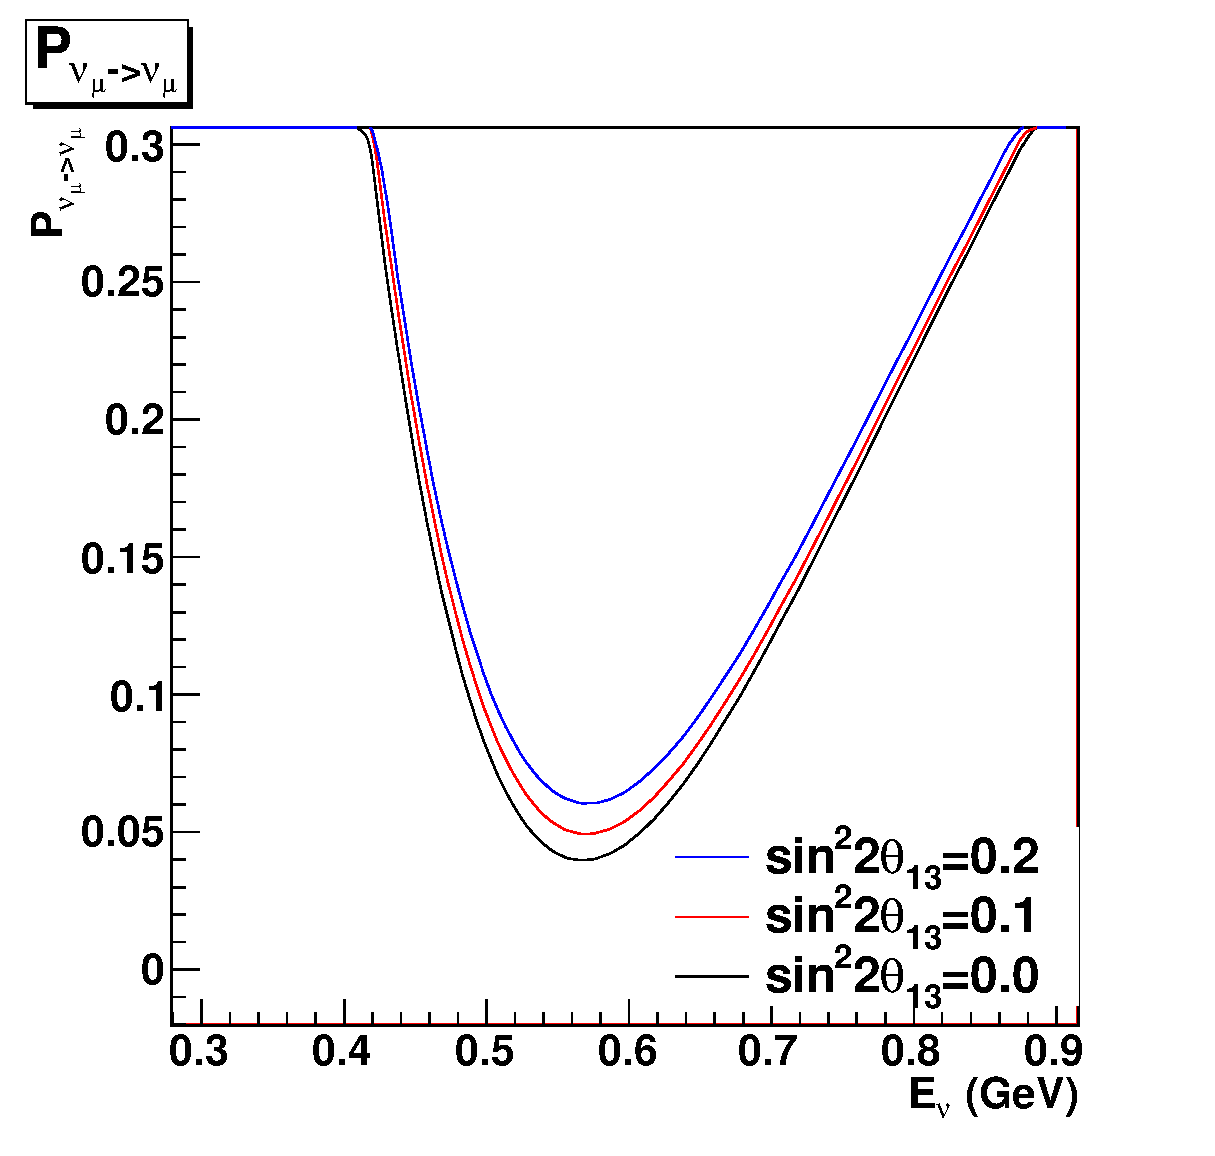
\includegraphics[width=0.45\textwidth]{images/motivation/OscProbNuMuNuMuZoom.eps}
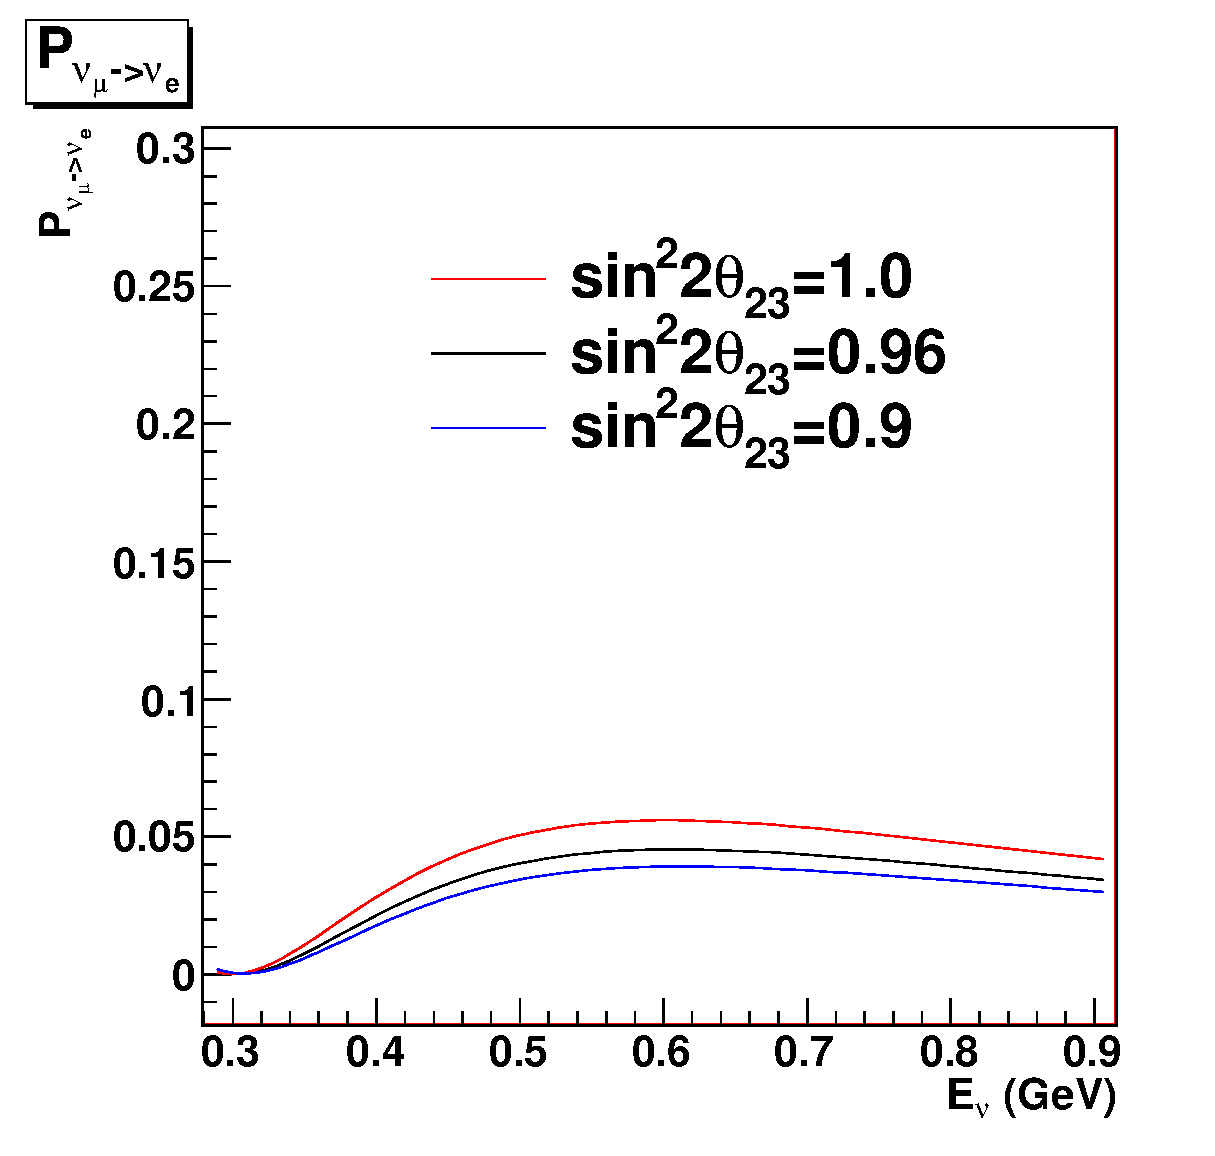
\includegraphics[width=0.45\textwidth]{images/motivation/OscProbNuMuNuEZoom.eps}
\caption{Examples of the effect of the interdependence between the oscillation parameters in the oscillation probabilities $P(\nu_{\mu}\rightarrow\nu_{\mu})$(left) 
and $P(\nu_{\mu}\rightarrow\nu_{e})$ (right). These probabilities are computed for different values of $\sin^{2}2\theta_{13}$ (left) or $\sin^{2}2\theta_{23}$ (right) 
with the other 3 parameters being fixed at $\sin^{2}2\theta_{23}$ = 0.96, $|\Delta m_{32}^{2}|$ = 2.4$\times$10$^{-3}$ eV$^{2}$/c$^{4}$, $\delta_{CP}$ = 0 (left) or 
$\sin^{2}2\theta_{13}$ = 0.1, $|\Delta m_{32}^{2}|$ = 2.4$\times$10$^{-3}$ eV$^{2}$/c$^{4}$, $\delta_{CP}$ = 0 (right).}
\label{fig:oscprob}
\end{center}
\end{figure}


\begin{figure}[htbp]
\begin{center}
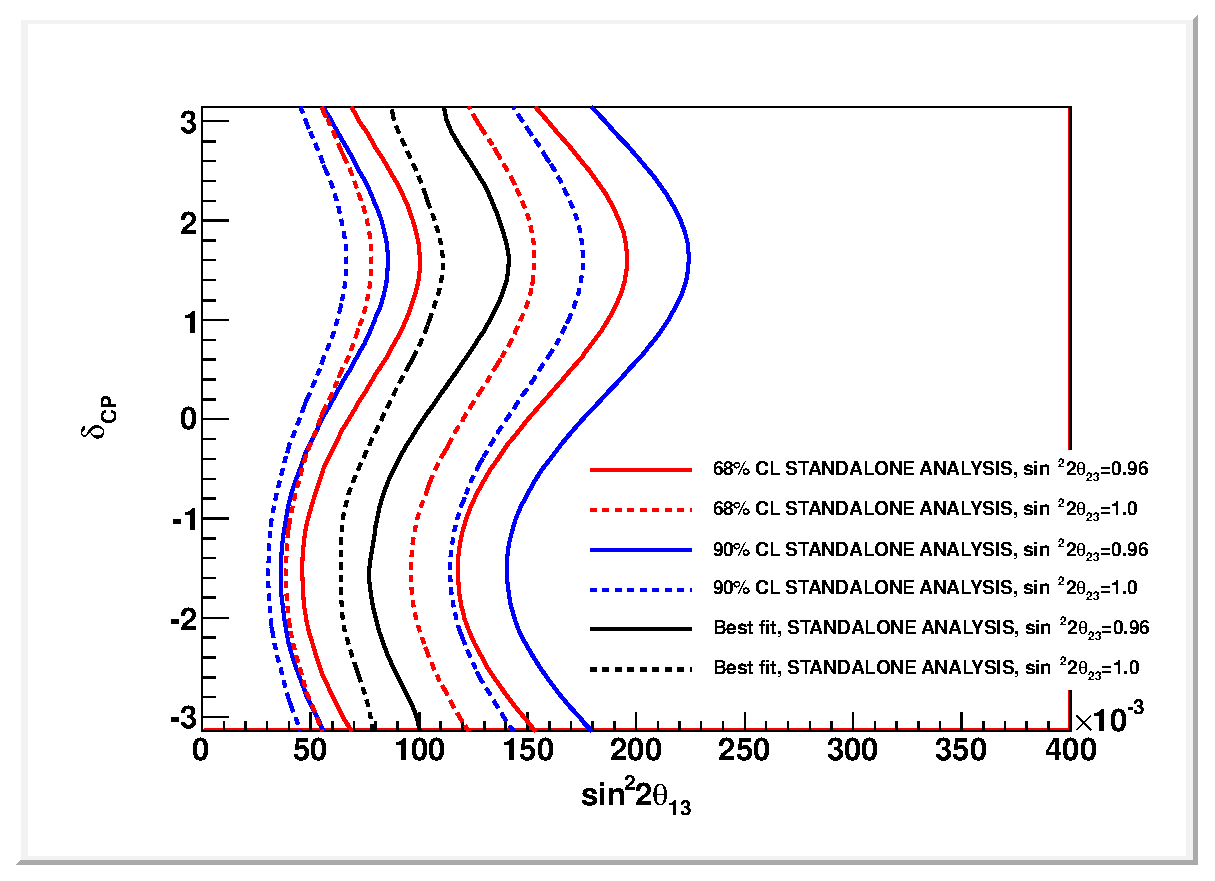
\includegraphics[width=0.7\textwidth]{images/motivation/ComparisonContoursStandaloneDifferentPriors.eps}
\caption{Illustration of the effect of changing the assumed value of $\sin^{2}2\theta_{23}$ in the $\nu_{e}$-appearance contours for 7$\times$10$^{21}$ POT. 
Dashed lines are contours of the stand-alone $\nu_{e}$-appearance analysis assuming maximal mixing ($\sin^{2}2\theta_{23}$ = 1.0), and solid lines are contours 
of the stand-alone $\nu_{e}$-appearance analysis assuming $\sin^{2}2\theta_{23}$ = 0.96, the true value with which the toy experiment was created. The other 
parameters have the following values: $\sin^{2}2\theta_{13}$ = 0.12, $|\Delta m_{32}^{2}|$ = 2.5$\times$10$^{-3}$ eV$^{2}$/c$^{4}$, and $\delta_{CP}$ = 0.5. 
The confidence regions were constructed using the constant-$\Delta\chi^{2}$ method, which is described in Sec.\ \ref{sec:neutrino_oscillation_fitting}.}
\label{fig:effectpriornuecontours}
\end{center}
\end{figure}

 
\begin{figure}[htbp]
\begin{center}
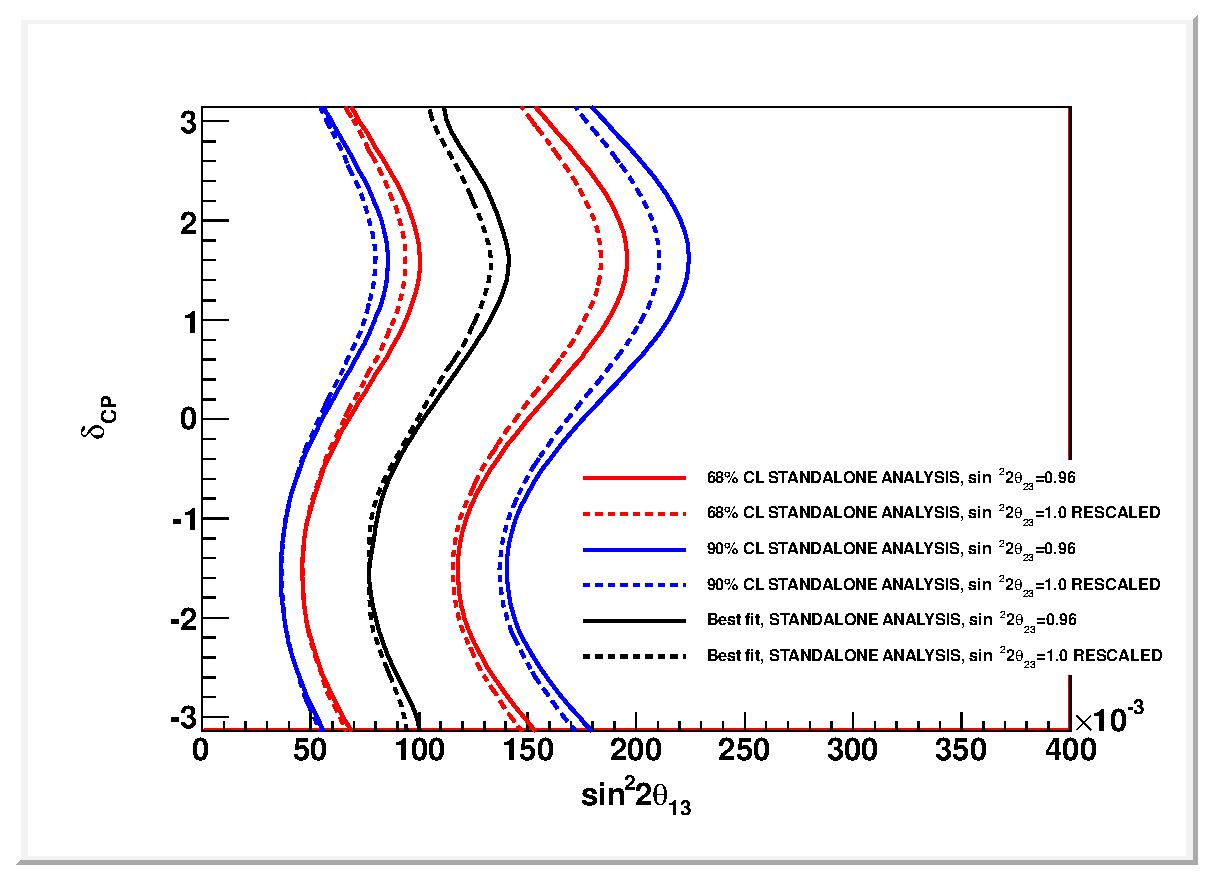
\includegraphics[width=0.7\textwidth]{images/motivation/ComparisonContoursStandaloneDifferentPriorsRescaling.eps}
\caption{Plot of the same contours as in Fig. \ref{fig:effectpriornuecontours} rescaling the contours for maximal prior $\sin^{2}2\theta_{23}$ = 1.0 with the cited 
replacement of $\sin^{2}2\theta_{13}$ by $2 \sin^{2}\theta_{23} \sin^{2}2\theta_{13}$, using for $\theta_{23}$ the true value for the toy experiment.}
\label{fig:comparisoncontoursrescaling}
\end{center}
\end{figure}



\clearpage
